% !TEX root = ../EjsS Manual.tex

\chapter{Adding ``Events'' in \Ejs}\label{chapter:JavascriptEJS}
\begin{center} 
\copyright~\emph{July 2011 by Larry Engelhardt} \\{\small Adapted and edited by Francisco Esquembre}
\end{center}

This document provides a description of ``events'' in EJS---both what they are and how they are added.

\section{What is the purpose of an ``event'' in EJS?}

The purpose of an ``event'' is to provide a way for a certain \emph{action} to occur (for example, pausing the simulation) at the exact instant that a certain \emph{condition} is met (for example, a ball hitting the ground).  For the example of a falling ball, the following lines of code can be used to implement the Euler algorithm: 
\begin{verbatim}[8]
y = y + v*dt; // Update the height, y (using the velocity)
v = v + a*dt; // Update the velocity, v (using the acceleration)
t = t + dt;   // Update the time, t (using the time step, dt)
\end{verbatim}

For the example of a ball \emph{hitting the ground}, the ``event'' is analogous to the following lines of code:
\begin{verbatim}[8]
if (y < 0)  // If the condition is true...
{           // then the code within {...} is executed
  _pause(); // This pauses the simulation.
}
\end{verbatim}

Note these lines of code pause this simulation when the ball hits the ground. (More precisely, this pauses the simulation \emph{after} the ball hits the ground.)  Using an event will accomplish the same purpose, but the use of an event will be superior to these lines of code in two ways:
\begin{enumerate}
\item The event will be more accurate than this code.
\item The event will be even simpler to create than this code.
\end{enumerate}

Using an event will be more \emph{accurate} than the lines of code listed above for the following reason.  The lines of code above are only executed at the discrete time steps $t=0$, $\Delta t$, $2\Delta t$, $3\Delta t$, $4\Delta t$, etc.  When using an event, EJS does much better than this.  If the height is found to change from a positive value to a negative value between $t=2\Delta t$ and $t=3\Delta t$, the ODEs will be re-evaluated (meaning that the height will be re-evaluated) at $t=2.5\Delta t$ (midway between the two times).  This will hence provide a better approximation to the \emph{actual} time that the ball hits the ground.  This process will then be repeated.  If the height is found to change from positive to negative between $t=2\Delta t$ and $t=2.5\Delta t$, the ODEs will be re-evaluated at $t=2.25\Delta t$ (the new midway point between the times). The number of times that this process is repeated is referred to as the number of \emph{iterations}, and since each iteration involves cutting the time interval in half, this method is referred to as the \emph{bisection} method.  After several iterations, this process should give a very accurate approximation to the exact moment that the event occurs.  (This process of finding precisely where a function crosses zero is generally referred to as \emph{root finding}.)

\section{How are events added in EJS?}

Creating an event in EJS is also very \emph{simple} to do. After creating a page of ODEs, an event can be added by clicking on the button labeled ``Events''.  After creating an event, a window will appear. This window is shown in Fig.~\ref{fig:appendixA/Events}.


\begin{figure}[htb]
  \centering
  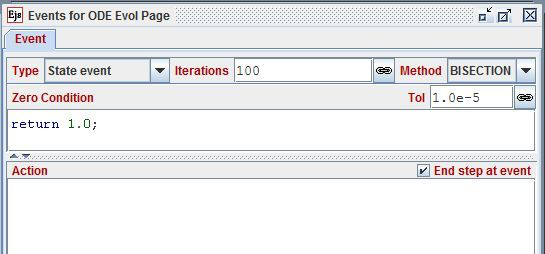
\includegraphics[scale=\scale]{appendixA/images/events_image.png}
  \caption{The blank page that appears when adding an event.}
  \label{fig:appendixA/Events}
\end{figure}

At the top of the window shown in Fig.~\ref{fig:events} several options can be specified. The menu in the top left corner allows you to choose the ``type'' of event to be used, as described in the following section. The maximum number of iterations (described in the previous section) can also be specified at the top of the page.  In the top right corner, the method of iteration can be selected.  The bisection method is described in the previous section.  The secant method is similar, but uses a secant line between the two points in time to estimate when the crossing event occurs.

Finally, it is necessary to specify the ``Zero condition'' and the ``Action''.  The zero condition consists of one or more lines of code, and it must include a \verb return ~statement. The quantity (or the \underline{\textbf{variable}}) following the word ``return'' will be checked to see whether or not the event has occurred (e.g., whether or not the ball has hit the ground).  For example, with the statement \verb+return 1.0;+ the event will never occur because 1.0 will always be greater than zero!  In fact, you would \emph{never} want to return a fixed numerical value because a fixed value can never change sign.  Hence, you need to replace the ``1.0'' with the thing that \emph{does} cross zero (and does change sign) at the moment that the event should occur.  One of the keys to using an event is to decide what quantity should follow the word \verb+return+.  The ``Action'' is the code to be executed when the event occurs, and it needs to be entered into the lower part of the window.

For the example of a ball hitting the ground, the \emph{event} can be described as ``the moment that the height crosses the value $y=0$''.  Hence, the \verb return ~statement would be \verb+return y;+.  This completed event is shown in Fig.~\ref{fig:appendixA/EventsComplete}.

\begin{figure}[htb]
  \centering
  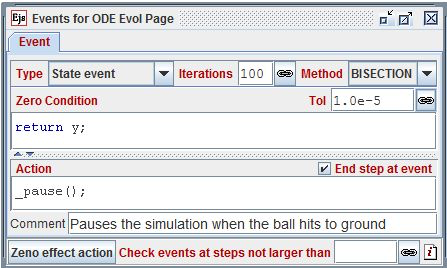
\includegraphics[scale=\scale]{appendixA/images/event_complete.png}
  \caption{The completed event that will pause the simulation when an object hits the ground.}
  \label{fig:appendixA/EventsComplete}
\end{figure}

\newpage
\section{Different ``types'' of events}

In the upper-left corner of the Event window (visible in Figs.~\ref{fig:events}~and~\ref{fig:events_complete}), you are able to choose between three different ``types'' of events:
\begin{enumerate}
\item State event
\item Zero crossing
\item Positive crossing
\end{enumerate}

Specifying the ``type'' of event to use can be a bit confusing for the following reason:  Your choice of which type of event to use \emph{doesn't matter}\ldots unless it does!  For example, the event shown in Fig.~\ref{fig:events_complete} that pauses the falling ball will work correctly regardless of which type of event is used.  In other situations though, the correct choice of event type can be very important.

Let us first consider the ``Zero crossing'' event.  This does exactly what you would expect.  When the value of the quantity specified by the \verb+return+ statement crosses zero, the event is triggered, and the \emph{Action} is executed.  The ``Positive crossing'' event does the same thing, except this type of event is \emph{only} triggered when the value of the quantity changes from positive to negative---not negative to positive.  Clearly either of these would work for the falling object, since---at the moment that it hits the ground---the height crosses zero \emph{and} changes sign from positive to negative.  As a different example, when using an event to measure the period of some type of oscillation, you might wish to use a \emph{positive} crossing rather than a \emph{zero} crossing.  This would allow you to measure the \emph{complete} period rather than only half an oscillation.  You might wonder why there is not a corresponding ``Negative crossing''.  Detecting a negative crossing is a very reasonable thing to want to do, and it is very easily accomplished:  Simply use a positive crossing, and include a negative sign after the word \verb+return+ in the Zero Condition!

The ``State event'' is just like the ``Positive crossing'' event, except that a \emph{state} event should be used in situations where it is \emph{not allowed} for the value of the quantity to be negative.  Examples could include objects \emph{bouncing} off of the ground, or off of a wall, or off of each other.  In these situations, you are \emph{required} to include code within the Action that will keep the quantity (following the \verb+return+) out of the ``forbidden region''.  For the examples of bouncing objects, this is accomplished by simply changing the sign of the velocities within the action.  For a concrete example of the difference between state events and positive crossing events, do the following:
\begin{enumerate}
\item Open the Event window shown in Fig.~\ref{fig:events_complete}, and remove (or comment out) the line of code that appears in the Action.  (Now the program will continue after the event is triggered.)
\item Run the program with \emph{State event} selected for the event type.  With a state event, negative values are not allowed, so you will see an error.  (This is EJS politely tapping you on the shoulder to let you know that you are ``breaking the rules''.)
\item Run the program again with either \emph{Zero crossing} or \emph{Positive crossing} selected for the event type.  Now there is no error, since negative values \emph{are} allowed for these types of events.
\end{enumerate}

As a final example, again select ``State event,'' but now specify \verb+v = -0.9*v;+ for the Action.  This will make the ball \emph{bounce}; but since the coefficient of restitution is less than 1, the maximum height of the ball will decrease (by the \emph{same fraction}) with each bounce.  We could now ask the question, ``How long will it take for the ball to come to rest?'' which is reminiscent of \emph{Zeno's paradoxes}.  To address these situations, click on the ``Zeno effect action'' button shown in the lower-left corner of Fig.~\ref{fig:events_complete}, and enter additional code to be executed in the event of infinitesimal bounces---e.g., pausing or resetting the simulation.



